\documentclass[12pt, twoside]{article}
\usepackage[letterpaper, margin=1in, headsep=0.5in]{geometry}
\usepackage[english]{babel}
\usepackage[utf8]{inputenc}
\usepackage{amsmath}
\usepackage{amsfonts}
\usepackage{amssymb}
\usepackage{tikz}
\usetikzlibrary{quotes, angles}
\usepackage{graphicx}
\usepackage{enumitem}
\usepackage{multicol}
\usepackage{hyperref}

\newif\ifmeta
\metatrue %print standards and topics tags

\title{IB Mathematics}
\author{Chris Huson}
\date{September 2021}

\usepackage{fancyhdr}
\pagestyle{fancy}
\fancyhf{}
\renewcommand{\headrulewidth}{0pt} % disable the underline of the header
\raggedbottom


\fancyhead[LE]{\thepage}
\fancyhead[RO]{\thepage \\ Name: \hspace{4cm} \,\\}
\fancyhead[LO]{BECA / IB Math 01-Linear functions\\* 21 September 2021}

\begin{document}

\subsubsection*{1.6 PreQuiz: Functions}
\begin{enumerate}
  \item Do Now: A trainer plans a pyramid workout routine. Let $x$ be the set number.
  \begin{center}
      Sample Bench Press Pyramid 
      (\href{https://www.bodybuilding.com/content/build-muscle-and-strength-with-pyramid-training.html}{Bill Geiger})\\
        Set 1: 135 lbs, 15 reps\\
        Set 2: 185 lbs, 12 reps\\
        Set 3: 205 lbs, 10 reps\\
        Set 4: 225 lbs, 8 reps\\
        Set 5: 245 lbs, 6 reps\\
        Set 6: 265 lbs, 4 reps
  \end{center}
\begin{enumerate}[itemsep=0.5cm]
  \item On the third set, when $x=3$, how much weight is lifted?
  \item On which set is the weight 245 pounds? \\(express your answer in the form $x=$ a number)
  \item Interpret the ordered pair $(2,185)$ in this context.\vspace{2cm}
  \item Does the weight increase by a constant amount with each set? Explain. \\(i.e. is the slope constant?) \vspace{1cm}
\end{enumerate}

\item Consider the function $f(x)=100 - 10x$.
\begin{enumerate}[itemsep=0.5cm]
  \item Write down the independent variable.
  \item Calculate $f(10)$ \vspace{1cm}
  \item Show that $f(4.5)=55$ \vspace{1.5cm}
  \item There is an $x$ for which $f(x)= -30$. Find this value of $x$.
\end{enumerate} \vspace{2cm}

\newpage

\item A relation composed of four points is plotted on the graph below, and represented as a set of ordered pairs as $\{ (-1,4),(2,3),(2,5),(4,3) \}$
\begin{multicols}{2}
\begin{enumerate}
  \item Write down the domain.
  \item Write down the range.
  \item What is the image of 4?
  \item Is the relation a function? Why or why not. \vspace{2cm}
\end{enumerate}
  \begin{center} %4 quadrant regents grid w T-Chart
  \begin{tikzpicture}[scale=0.8]
    %\draw [help lines] (-3,-2) grid (4,6);
    \draw [thick, ->] (-3.2,0) -- (5.4,0) node [below right] {$x$};
    \draw [thick, ->] (0,-1.2)--(0,6.4) node [left] {$y$};
    \foreach \x in {-2, -1, ..., 5} \draw (\x cm,1pt) -- (\x cm,-1pt) node[anchor=north] {$\x$};
    \foreach \y in {1, 2, 3, 4, 5} \draw (1pt,\y cm) -- (-1pt,\y cm) node[anchor=east] {$\y$};
    %\draw [thick, <->] (-3.5,-1.5) -- (4.2,6.2);
    \fill (-1,4) circle[radius=0.1] node[above left]{$(-1,4)$};
    \fill (2,3) circle[radius=0.1] node[above]{$(2,3)$};
    \fill (2,5) circle[radius=0.1] node[above]{$(2,5)$};
    \fill (4,3) circle[radius=0.1] node[above right]{$(4,3)$};
  \end{tikzpicture}
  \end{center}
\end{multicols}
\vspace{0.25cm}

\item An investor owns a building with five apartments. She calculates the monthly profit depending on the number of apartments rented, shown in the table. 
\begin{center}
  \begin{tabular}{|l|r|r|r|r|r|r|}
    \hline
    Units rented & 0 & 1 & 2 & 3 & 4 & 5\\ 
    \hline 
    Profit(\$000) & -85 & -70 & -40 & -10 & 20 & 50\\ 
    \hline 
  \end{tabular}
\end{center}
\begin{enumerate}
  \item What is her profit if the building is fully rented?\vspace{0.25cm}
  \item How many apartments must be rented in order not to lose money?\vspace{0.25cm}
  \item Is her profit linear? (does it increase by a constant amount with each apartment?) Explain why or why not in the context of the situation.
\end{enumerate} \vspace{2cm}


\item The graph of a function $f$ is shown on the grid below.
\begin{multicols}{2}
\begin{enumerate}
  \item What is $f(3)$?
  \item Write down the domain.
  \vspace{0.25cm}
  \item Write down the range. \vspace{0.5cm}
\end{enumerate}
  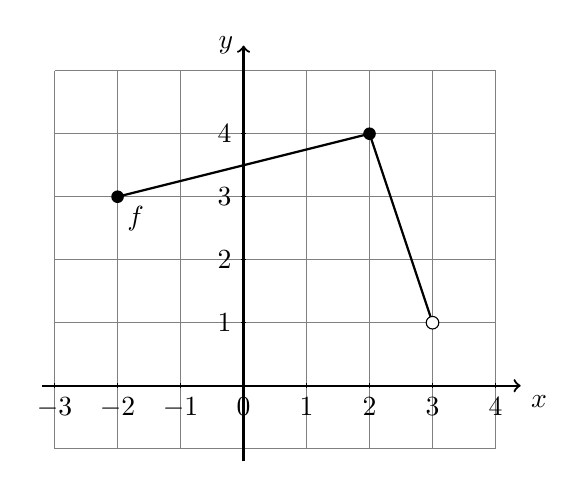
\begin{tikzpicture}[scale=0.8]
    \draw [help lines] (-3,-1) grid (4,5);
    \draw [thick, ->] (-3.2,0) -- (4.4,0) node [below right] {$x$};
    \draw [thick, ->] (0,-1.2)--(0,5.4) node [left] {$y$};
    \foreach \x in {-3, -2, ..., 4} \draw (\x cm,1pt) -- (\x cm,-1pt) node[anchor=north] {$\x$};
    \foreach \y in {1, 2, 3, 4} \draw (1pt,\y cm) -- (-1pt,\y cm) node[anchor=east] {$\y$};
    \draw [thick] (-2,3) -- (2,4) -- (3,1);
    \fill (-2,3) circle[radius=0.1] node[below right]{$f$};
    \fill (2,4) circle[radius=0.1];
    \fill [white] (3,1) circle[radius=0.1];
    \draw (3,1) circle[radius=0.1];
  \end{tikzpicture}
\end{multicols}

\end{enumerate}
\end{document}